\documentclass[conference]{IEEEtran}
\include{psfig}
\include{epsfig}
\usepackage{algorithm}
\usepackage{algorithmic}
\usepackage{rotating}
\usepackage{fontenc}
\usepackage{graphicx}
\usepackage{amsfonts}
\usepackage{amsmath}
\usepackage{cite}
\usepackage{proba}
\usepackage{amssymb,latexsym}
\usepackage{subfigure}
\usepackage{graphicx}
\usepackage{dsfont,multirow}
\usepackage{float}
%\interdisplaylinepenalty=2500

\newcommand{\be}{\begin{equation}}
\newcommand{\ee}{\end{equation}}
\newcommand{\bd}{\begin{displaymath}}
\newcommand{\ed}{\end{displaymath}}
\newcommand{\bear}{\begin{IEEEeqnarray}}
\newcommand{\eear}{\end{IEEEeqnarray}}
\newcommand{\bo}[1]{\textbf{\emph{#1}}}


\newtheorem{lem}{Lemma}
\newtheorem{defn}{Definition}
\newtheorem{prop}{Property}
\newtheorem{prosi}{Proposition}
\newtheorem{thm}{Theorem}
\newtheorem{exmp}{Example}
%\usepackage{tikz}
%\usetikzlibrary{backgrounds}	% drawing the background after the %foreground
%\usetikzlibrary{shapes.geometric}
%\usepackage{enumitem}
%\let\labelindent\relax
%\newcommand{\keywords}[1]{\par\addvspace\baselineskip
%\noindent\keywordname\enspace\ignorespaces#1}



%\usepackage{here}

% LLNCS model

\begin{document}
\title{Mathematical methods for analyzing performance and energy consumption in the cloud}


%\title{Mathematical methods for performance analysis of hysteresis queues}
%\thanks{partially supported by French research project ANR-MARMOTE}

%\numberofauthors{4}

% \author{
% \IEEEauthorblockN{M. Kandi}
% \IEEEauthorblockA{SAMOVAR, CNRS, Telecom SudParis\\
% Université Paris-Saclay\\
% 9, rue Charles Fourier, 91011 Evry Cedex, France \\
% Email: medmehdikandi@gmail.com}
% \and
% \IEEEauthorblockN{F. {A\"{\i}t-Salaht}}
% \IEEEauthorblockA{
% LIP6, Crest-Ensai, Rennes, France\\
% Email: farah.ait-salaht@ensai.fr
% }
% 
% \and
% \IEEEauthorblockN{H. Castel-Taleb}
% \IEEEauthorblockA{SAMOVAR, CNRS, Telecom SudParis\\
% Université Paris-Saclay\\
% 9, rue Charles Fourier, 91011 Evry Cedex, France \\
% Email: hind.castel@telecom-sudparis.eu}
% \and
% \IEEEauthorblockN{E. Hyon}
% \IEEEauthorblockA{Sorbonne Universit{\'e}s, UPMC Univ Paris 06,\\
% CNRS, LIP6 Paris UMR 7606, \\
% 4 place Jussieu 75005 Paris}
% \IEEEauthorblockA{Universit{\'e} Paris Nanterre\\
% Email: emmanuel.hyon@lip6.fr}
% }



\author{
\IEEEauthorblockN{M. Kandi \IEEEauthorrefmark{1}, 
F. {A\"{\i}t-Salaht}\IEEEauthorrefmark{2} \IEEEauthorrefmark{3},
H. Castel-Taleb \IEEEauthorrefmark{1}, 
and
E. Hyon \IEEEauthorrefmark{3} \IEEEauthorrefmark{4}
}
\IEEEauthorblockA{\IEEEauthorrefmark{1}
SAMOVAR, CNRS, Telecom SudParis, Universit{\'e} Paris-Saclay\\
9, rue Charles Fourier, 91011 Evry Cedex, France \\
Email: medmehdikandi@gmail.com, hind.castel@telecom-sudparis.eu
}
\IEEEauthorblockA{\IEEEauthorrefmark{2}
Crest-Ensai, Rennes, France\\
Email: farah.ait-salaht@ensai.fr
}
\IEEEauthorblockA{\IEEEauthorrefmark{3}
Sorbonne Universit{\'e}s, UPMC Univ Paris 06, CNRS, LIP6 Paris UMR 7606, \\
4 place Jussieu 75005 Paris}
\IEEEauthorblockA{\IEEEauthorrefmark{4} Universit{\'e} Paris Nanterre\\
Email: emmanuel.hyon@lip6.fr}
}


\maketitle


\begin{abstract}
We propose in this paper to evaluate using mathematical methods the performance and the energy consumption of cloud system.
We consider for the analysis an hysteresis queueing system, which is characterized by forward and backward thresholds for
activation and deactivation of block of servers representing a set of VMs (Virtual Machines).
The system is represented by a complex Markov Chain which is difficult to analyze when the size of the system is huge.
For this case, we propose three different mathematical methods for computing the steady-state probability distribution:
the SCA (Stochastic Complement Analysis) method in order to aggregate
the state space, Level Dependent Quasi Birth and Death (LDQBD) method, and the balance equations that allows to derive exact formulas
for the steady-state probability distribution.
We compute both performance and energy consumption measures and we define an overall cost taking into account both aspects.
Then these three methods are compared from their computation time. Moreover, we analyze the impact of some parameters
as the thresholds, and the arrival rate on the behavior of the system.
\end{abstract}


\section{Introduction}

Recently, Cloud computing has changed the way people do computing and manage information, since 
a pool of  virtualized, dynamically-scalable computing functions and services are made accessible over the internet
to remote users in an on-demand fashion. With virtualization, the cloud providers can adapt the virtual machines
according to the demand, and   service providers can  provide resources in
a cost-effective manner by consolidating VMs onto fewer physical resources when system load is low,
and quickly scale up workloads to more physical resources when system load is high.

Finding the policy that tailors resources to demand is a crucial point in such systems.
Multi server queuing models \cite{Artalejo2005} or server farms models \cite{Gandhi2010,mitrani2013managing} have been proposed
since they are well suited to represent the behavior of a data center and its dynamicity as well as to compute its performance metrics.
In such models the servers can be activated and deactivated either   server by server or by blocks of servers  according to the intensity 
of user demand.
A special case of model is the multi-server threshold based-queueing system with hysteresis policy \cite{art:serfozo}, in which activations 
and deactivations are governed by sequences of forward and reverse different thresholds
where each time the workload (or the number of customers in the system) reaches a forward or reverse thresholds only one server (here one VM)
is activated or deactivated. We propose in this paper to extend the current state of art and
to couple the advantages of the activation by block and the advantages of hysteresis policy
by considering a multi-server system with hysteresis in which
activation/deactivation are made by block (ie. activate or deactivate at same time a set of VMs).
This to our knowledge has never been considered and studied previously in the literature. Moreover, in this paper, 
one objective is to consider both performance and energy consumption in order to propose a tradeoff between them. 

The assessment of both performance and  energy consumption of cloud system driven by hysteresis policies requires
the computation of the expected measures. But we face up a computational complexity problem since cloud systems are often defined
on very large state spaces which makes their exact analysis very cumbersome or even impossible.
Under some considerations and assumptions, this problem has been already studied in the literature
and different resolution methods have been presented to compute efficiently (in exact and less complex manner) the performance measures of the system.
Among the most significant works, we can mention the work of Lui and Golubchik \cite{lui1999stochastic} which
solves the model, using the concept of stochastic complementation. This method is based on partitioning the state space
in disjoint sets in order to aggregate the Markov chain.  The main advantage of this method is to obtain exact performance results, with reduced
execution times. In \cite{le2000simple}, Le Ny et al. propose to compute the steady-state probabilities of a heterogeneous multi-server threshold queue
with hysteresis by using a closed-form solution.  Finally in  \cite{ait2016mascots}, the authors analyze the system through stochastic
bounding theory and define accurate bounds on performance measures.
However, in these works, we emphasize that they considered only the case where one VM is activated (resp. deactivated)  according to
the demand and the threshold sequences.  

In this work we investigate the problem when activation and deactivation are done by blocks and present some proved analysis and resolution methods.
We first adapt and extend the SCA (Stochastic Complement Analysis) method in order to aggregate
the state space and we couple it with a numerical resolution method (such as GTH method \cite{Stew95}) to improve the efficiency.
Furthermore, we propose an analytical approach by  adapting the balance equations method of \cite{le2000simple} and we get exact formulas 
for the steady-state probability distribution.
We also extend the method by relaxing the former assumptions on the thresholds that \cite{le2000simple} made. 
At last, a numerical approach based on Level Dependent Quasi Birth and Death (LDQBD) method is presented in details. 
This last one is the closest of usual resolution methods
and allows to know the improvement brought by the two previous ones. We obtain numerical results even for large Markov chains,
and we establish an overall cost taking into account both performance and energy consumption. Moreover, as we consider 
in this model more general assumptions for the thresholds, then  we can  see in details the impact of their  values 
on performance and energy consumption.  


The paper is organized as follows: next (section \ref{sec:ModelDet}), we describe the cloud system and present the considered queueing model
for the analysis. In section \ref{sec:ResModel}, we detail the different methods to solve the model and compute the steady state probability vector.
While \ref{sec:ParamPerf} presents the formulation used to express the expected costs
in terms of performances and energetic consumption for the model,
section \ref{sec:ResNum} presents numerical results of  performance and energy consumption measures. Finally, 
achieved results are discussed in the conclusion and comments about further research issues  are given.


\section{Cloud system description} \label{sec:ModelDet}

We analyse  a cloud system composed by a set of Virtual Machines (VMs). We assume that the job requests arrive at the system
following a Poisson process with rate $\lambda$, and are enqueued in a finite queue with capacity $B$. An arriving request can be rejected if
it finds the buffer full.
We model this system  using a multi-server queue,  with $C$ homogeneous servers representing the VMs. The service time of each VM  is exponential
with mean rate $\mu$. In order to represent the dynamicity of resource provisioning, the VMs are activated and deactivated according to the system
occupancy. Actually, the buffer management is governed by thresholds vectors corresponding to the number of customer waiting in the system, which
controls the operation of activating and deactivating the VMs. We suppose the case where the VMs are activated or deactivated by block, which means
that several VMs can be simultaneously activated or deactivated.

We define   $K$ functioning levels, where each level corresponds to a given number of active servers. The number of active servers at level $k$ is
fixed and denoted by $S_k$, where $S_{1} \leq S_{2} \leq ... \leq S_{K}=C$. We suppose that $S_1 \geq 1$, so we have  at least  
one active server by assumption. The transition from functioning level $k$ to level $k+1$ allows to allocate (turn on) one or more additional servers, going from
$S_k$ to $S_{k+1}$ active servers, while the transition from level $k$ to level $k-1$ allows to remove (turn off) one or more active servers,
going from $S_k$ to $S_{k-1}$ active servers. Depending on the system occupancy, we transit from the level $k$ to level $k+1$ when the occupancy in
the system exceeds a threshold $F_{k}$, and from level $k$ to level $k-1$ when the occupancy in the system falls below a threshold  $R_{k-1}$.
The model is then characterized by activation thresholds  $F=(F_{1}, F_{2}, ..., F_{K-1})$ (called also forward thresholds), and deactivation
thresholds $R=(R_{1}, R_{2}, ..., R_{K-1})$ (called also reverse thresholds).
These thresholds are fixed and can not be modified during the system works.
We furthermore assume  that $F_{1}<F_{2}< ...<F_{K-1}$, that $R_{1}<R_{2}< ...<R_{K-1}$ and that $R_{k}<F_{k}, \forall k, 1 \leq k \leq K-1$.
We suppose here that server deactivations occur at the end of the service, and when multiple servers are deactivated at the same times,
all the customers who have not completed their service return to the queue.

The underlying model is  described by the Continuous-Time Markov Chains (CTMCs), denoted   $\{X(t)\}_{t \geq 0}$.
A state is represented by a couple $(m,\,k)$ such that $m$ is the number of customers in the system and $k$ is the functioning level.
The state space is denoted by $A$ and is given as follows:
\begin{align*}
A=\{(m,\,k) \, | \,  & 0 \leq m \leq F_{1},  \text{ if } k=1 ; \\
                           & R_{k-1}+1 \leq m \leq F_{k}, \text{ s.t. } 1 < k < K ; \\
                           & R_{K-1}+1 \leq m \leq B,  \text{ if } k=K;
\}
\end{align*}
Recalling that   $S_{k}$ represents the number of active servers at level $k$, the transitions between states follows:
\begin{equation*}
\begin{array}{rcl}
\! \! (m,\,k)\! & \! \rightarrow & (\min\{B,m+1\},\,k) \; \text{with rate } \lambda \, , \text{ if } m < F_{k} ;\\
                & \! \rightarrow & (\min\{B,m+1\},\,\min\{K,\,k+1\}) \\
                & & \! \text{with rate } \lambda, \, \text{ if } m=F_{k} ; \\
                & \! \rightarrow &  (\max\{0,m-\!1\},\,k), \text{with rate} \, \min\{S_{k},\,m\} \! \cdot \! \mu,    \\
                & & \! \text{if } m \! > R_{k-1} \!+\! 1  ; \\
                & \! \rightarrow & (\max\{0,m-1\},\,\max\{1,k-1\}) \\
                & & \! \text{with rate }   \min\{S_{k},\,m\} \cdot \mu,    \\
                & & \! \text{if }   m=R_{k-1}+1  \, .
\end{array}
\end{equation*}
An example of the transitions is given Figure \ref{fig:image-chap4-exemple_par_bloc}.

\begin{figure}[hbtp]
\centering
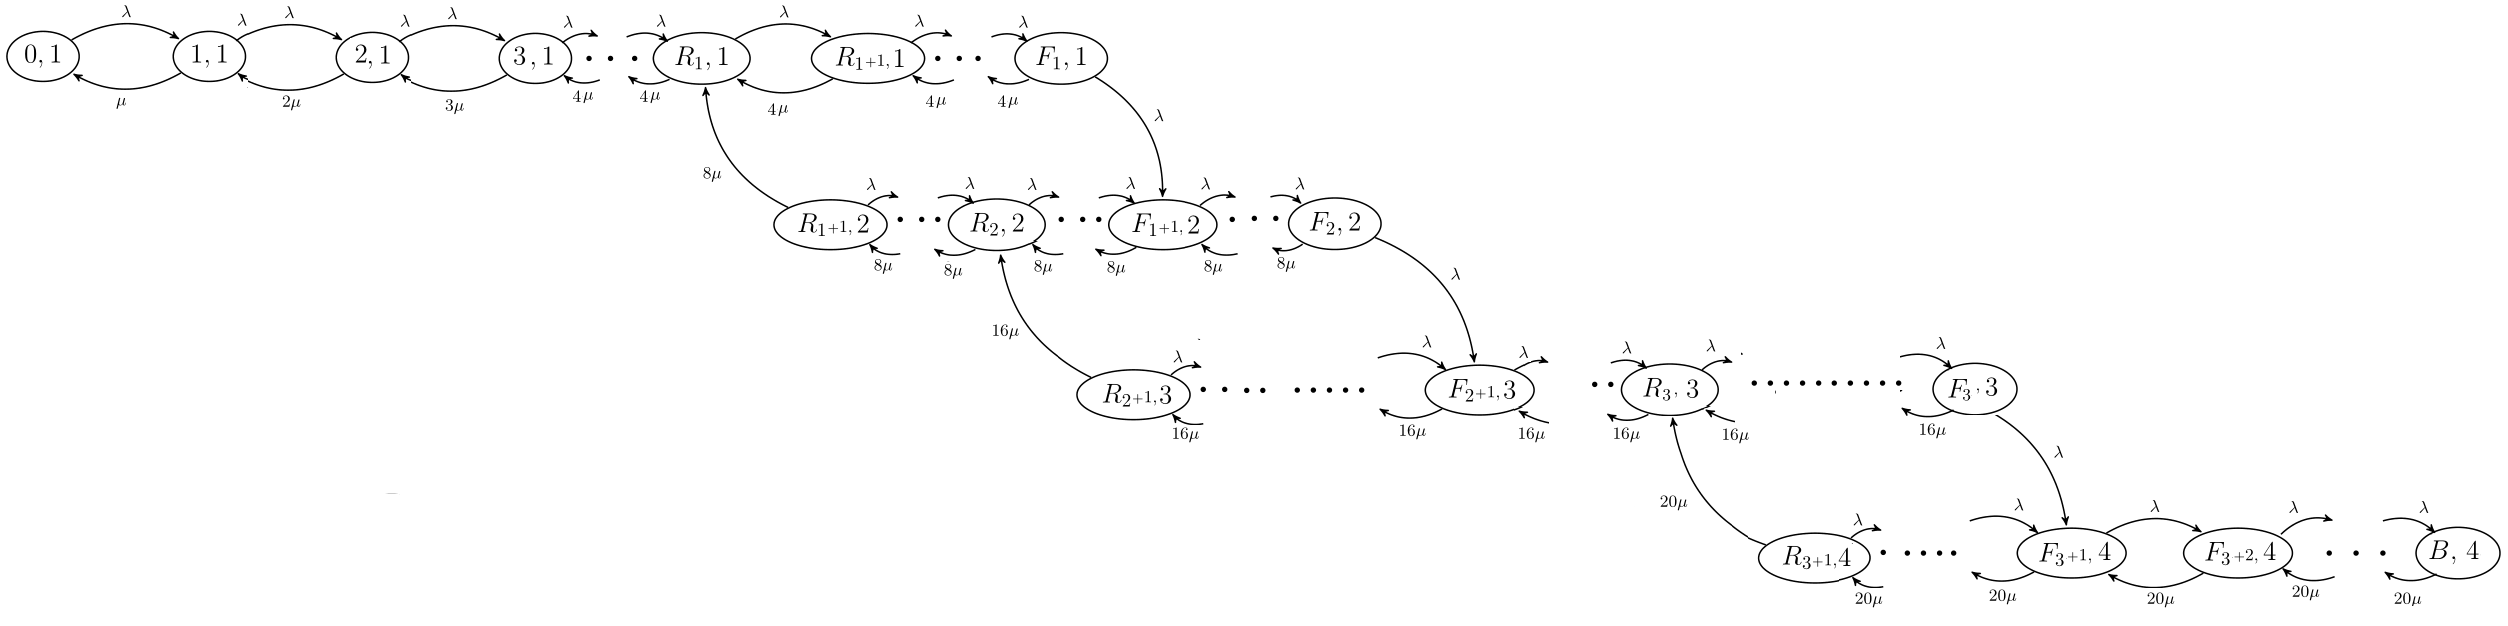
\includegraphics[width=0.47\textwidth, height=0.23\textwidth,]{images/exemple_par_bloc3.png}
\caption{Transition structure for $K=4$, $S_1=4$, $S_2=8$, $S_3=16$, $S_4=20$, $R_1+1 \geq 8$, $R_2+1 \geq 16$ and $R_3+1 \geq 20$.}
  \label{fig:image-chap4-exemple_par_bloc}
\end{figure}



\section{Resolution approaches} %//Farah
\label{sec:ResModel}
In order to compute the performance measures of the presented models, we expose hereafter some techniques to solve the CTMC and compute 
the steady state probability vector. Three resolution methods, either numerical or analytical, 
developed for this model are given and their comparisons in terms of execution times appear in Section~\ref{sec:ResNum}.

\subsection{Stochastic Complement Analysis (SCA)} %//Farah

\label{sec:SCA}
To solve the $\{X(t)\}_{t \geq 0}$ Markov chain, the first approach consists to aggregate the underlying chain and use a numerical method to compute 
the steady state distribution. This approach has been proposed by Lui et al. \cite{lui1999stochastic}
and works as follows. First, we aggregate the state space of the underlying Markov chain by partitioning the set $A$ into disjoint subsets. 
The number of derived subsets depends on the number of functioning level. From each subset, we define a corresponding Markov chain. 
These derived Markov chains are defined on reduced state spaces which makes their analysis less complex. 
The resolution of each Markov chain defines a conditional steady state probabilities.
By applying the state aggregation technique, each subset is now represented by a single state, and an aggregated process is defined. 
A resolution of this aggregated process is performed, i.e., the probabilities of the system being in any given set are computed. 
We note that the compute of the steady state probabilities of a Markov chain can be obtained using any chosen solution technique, 
as described in \cite{Stew95}.
Lastly, a disaggregation technique is applied to compute the individual steady state probabilities of the original Markov process.

 %solved through a well-known numerical technique GTH \cite{grassmann1985regenerative}.

In the following, we present an important theorem stated by  Lui et al.   in their article \cite{lui1999stochastic}.%which is a more intuitive and more easily extensible method
\begin{thm}[\cite{lui1999stochastic}]
\label{thm:thm1}
Given an irreducible Markov process with state space $A$, let us partition this state space into two disjoint set $A_1$ and $A_2$. 
Then, the transition rate matrix (denoted by $Q$) is given as follows:
\begin{equation*}
Q = \left(\begin{IEEEeqnarraybox*}[][c]{,c/c/c,}
    Q_{A_{1}A_{1}}       & Q_{A_{1}A_{2}} \\
    Q_{A_{2}A_{1}}       & Q_{A_{2}A_{2}} %
\end{IEEEeqnarraybox*}\right),
\end{equation*}
where $Q_{i,j}$ is the transition rate sub-matrix corresponding to transitions from partition $i$ to partition $j$.
\end{thm}

Based on this theorem and under some restrictions, Lui et al. have investigated the case where we activate (resp. deactivate) only one server  
when the number of customers in the system reaches a forward or reverse threshold. Here, and without any restrictions, we propose to give a general 
formulation for the multi-server threshold based-queueing system with hysteresis  where activation and deactivation are made by block.

So, given the $\{X_{t}\}_{t \geq 0}$ Markov chain with state space $A$,  we partition the state space  $A$ into $K$ distinct sets 
denoted $A_{k}$, $1 \leq k \leq K$, where:
\begin{equation}
A_{k}=\{(i,\,j)|(i,\,j) \in A \mbox{ and } j=k\}; \, \forall \, k=1...K 
\end{equation}
The set $A_{k}$ contains the states belonging the level $k$.

Let $\{(X_{k})_{t}\}_{t \geq 0}$ be a Markov chain defined on state space $A_{k}$, $\forall k=1...K$. 
We denote by  $\pi_{k}$ the steady state probabilities of $X_{k}$. 
The transitions in $\{(X_{k})_{t}\}_{t \geq 0}$ are identical to those appearing in the original process $\{X_{t}\}_{t \geq 0}$ 
for the level $k$ except some additional modifications that are set out below:

For $k=1$. We add a transition from state $(F_{1},1)$ to state $(R_{1},1)$ with a rate $\lambda$.

For $k \in \{2,\ldots,K-1\}$:  we add a transition from state $(F_{k},\,k)$ to state $(R_{k},\,k)$, 
with a rate $\lambda$, and we add transition from $(R_{k-1}+1,\,k)$ to state $(F_{k-1}+1,,)$, with a rate ($\min\{R_{k-1}+1,S_k\} \cdot \mu$).

For $m=K$: we add a transition from state $(R_{K-1}+1,\, K)$ to state $(F_{K-1}+1,\,K)$, with a rate $\min\{R_{K-1}+1,S_K\} \cdot \mu$.

Besides, the aggregated process that brings all aggregate states is a simple birth and death process, with:
\begin{itemize} %% on peut gagner de la place ici au cas ou
\item $\lambda_{k}$=$\lambda \cdot \pi_{i}(F_{k})$,\;\; $\forall k=1\cdots K-1$ 
\item $\mu_{k}$=$ \mu \cdot \min(R_{k-1}$+$1,S_k) \cdot \pi_{k}(R_{k-1} + \!1)$,\; $\forall k=2\cdots K$.
\end{itemize}
We denote by $\overline{\pi}$ the steady state probabilities of this aggregated process.
%through this aggregation, the compute of the steady state vector  of the original process, is now less complex. 
it consists to multiply the steady state vectors of the micro-chains with  the probabilities vector of the aggregated .


At this point we have all the necessary informations to compute the steady probabilities of $\{X_{t}\}_{t \geq 0}$. 
Indeed, we determine: (1) for each level $k$ ($k=1\ldots K$), the conditional state probabilities of all states $\pi_k$, 
and (2) the steady state probability of the aggregated process $\overline{\pi}$. 
Hence, the steady state probability of each individual state $(i,j)\in A$,  can be expressed as:
\(
\pi(i,\,j)=\pi_j(i)\,\overline{\pi}(j)\;\; \mbox{where} \;\; (i,\,j)\in A_j.
\)


\subsection{Level Dependant Quasi Birth and Death Process}

The particular form of the generator of $\{X(t)\}$ suggest us to use the Quasi Birth and Death (QBD) processes in order to benefits of the numerous
existing numerical methods to solve them \cite{Neuts1981}. For short, a QBD process is a stochastic process in which the state space is two dimensionals 
and can be decomposed in disjoint sets such that transition may only occur inside a set or occur towards only two other sets.
This results in a generator with a tridiagonal form (as the birth and death process) in which the terms on the diagonals are matrices.
When the matrices are identical for each level it is said \emph{level independant} but when the matrices are different the QBD
is said \emph{level dependant} (LDQBD).


Let us define $Q_{k,k'}(i,j)$ that denotes the $i$-th line and $j$-th column element of matrix $Q_{k,k'}$. We have

\begin{prosi}
The Markov Chain $\{X_{t}\}_{t \geq 0}$ %defined in section~\ref{sec:ModelDet} 
is a Level Dependant QBD with $K$ levels, corresponding to the functioning levels. Its generator $Q$ can be decomposed in :
\begin{equation*}
Q \! = \!  \left(\begin{IEEEeqnarraybox*}[][c]{,c/c/c/c/c/c,}
    Q_{1,1} & Q_{12,} & & & &  \\
    Q_{2,1} & Q_{2,2} & Q_{2,3} & & &  \\
     & Q_{3,2} & Q_{3,3} & Q_{3,4} & &  \\
    & & \ddots & \ddots & \ddots &  \\
    & & & Q_{K-1,K-2} & Q_{K-1,K-1} & Q_{K-1,K} \\
    & & & & Q_{K,K-1} & Q_{K,K}%
\end{IEEEeqnarraybox*}\right)\, .
\end{equation*}
For all $k$, the inner matrices $Q_{k,k-1}$, $Q_{k,k}$ and $Q_{k,k+1}$ are respectively of dimension  $d_{k} \times d_{k-1}$, $d_{k} \times d_{k}$ 
and $d_{k} \times d_{k+1}$, letting $d_{k}=F_{k}-R_{k-1}$, $R_{0}=-1$ and $F_{K}=B$.

For $k=1$ we have:
\begin{equation*}
Q_{1,1}(i,j)=
\begin{cases}
\lambda                   & \mbox{if } j=i+1\\
\mu \min\{S_{1},i\}       & \mbox{if } j=i-1\\
- \lambda                  &  \mbox{if } i=1 \mbox{ and } j=1\\
- (\lambda+ \mu \min\{S_{1},i\}) & \mbox{if } i=j \mbox{ and } i \neq 1\\
0                                & \mbox{otherwise}%
\end{cases}\, ,
\end{equation*}
and
\begin{equation*}
Q_{1,2}(i,j) =
\begin{cases}
\lambda & \text{if } i=d_1 \text{ and } j=F_{1}-R_{1}+1\\
0       & \text{otherwise}
\end{cases}\, .
\end{equation*}

For $k \in {2,....K-1}$, we get:
\begin{multline*}
Q_{k,k-1}(i,j)= \\
\quad \, 
\begin{cases}
\mu \min\{S_{k},R_{k-1}\!+\!1\}  & \text{if } i= \! 1 \text{ and } j \! = \! R_{k-1} \! - \! R_{k- \! 2}\\
0 & \text{otherwise}
\end{cases}\, ,
\end{multline*}
also
\begin{equation*}
Q_{k,k}(i,j) =
\begin{cases}
\lambda                                 & \text{if } j=i+1\\
\mu \min\{S_{k},R_{k-1}+i\}             & \mbox{if } j=i-1\\
-(\lambda+\mu \min\{S_{k},R_{k-1}+i\})  & \text{if } i=j\\
0                                       & \text{otherwise}
\end{cases}\, ,
\end{equation*}
and
\begin{equation*}
Q_{k,k+1}(i,j) =
\begin{cases}
\lambda             & \text{if } i=d_{k} \text{ and } j=F_{k}-R_{k}+1\\
0                   & \mbox{otherwise}
\end{cases}\, .
\end{equation*}
%\begin{equation}
% \setlength{\nulldelimiterspace}{0pt}
% Q_{i,i-1}(j,k) =\left\{\begin{IEEEeqnarraybox}[\relax][c]{l's}
%         min\{S_{i},R_{i-1}+1\}*\mu & $\mbox{si } j=1 \mbox { et }$ \\
% 				& $k=R_{i-1}-R_{i-2}$\\
%         %-(min\{S_{i},R_{i-1}+1\}*\mu) &\mbox{si } j=k=1\\
%         0 &\mbox{sinon}
% \end{IEEEeqnarraybox}\right.
% \end{equation}

% \begin{equation}
% \setlength{\nulldelimiterspace}{0pt}
% Q_{i,i}(j,k) = \left\{\begin{IEEEeqnarraybox}[\relax][c]{l's}
%         \lambda & \mbox{si } j+1=k\\
%         min\{S_{i},R_{i-1}+j\}*\mu & \mbox{si } j=k+1\\
%         -(\lambda+min\{S_{i},R_{i-1}+j\}*\mu) &\mbox{si } j=k\\
%        0 & \mbox{sinon}
% \end{IEEEeqnarraybox}\right.
% \end{equation}
%
% \begin{equation}
% \setlength{\nulldelimiterspace}{0pt}
% Q_{i,i+1}(j,k) = \left\{\begin{IEEEeqnarraybox}[\relax][c]{l's}
%         \lambda & $\mbox{si } j=d_{i} \mbox{ et } k=F_{i}-R_{i}+1$\\
%        %-\lambda & \mbox{si } j=k=F_{1}+1\\
%         0 & \mbox{sinon}
% \end{IEEEeqnarraybox}\right.
% \end{equation}

Finally for $k=K$, it follows
\begin{multline*}
Q_{K,K \!-\!1}(i,j) = \\
\quad
\begin{cases}
\mu \min\{S_{K},R_{K \!-\!1} \!+\!1\}   & \! \mbox{if} \, \, i\!=\!1 \, \, \mbox{and} \, \,  j\!=\!R_{K \!-\!1}\!-\!R_{K\!-\!2}\\
0                                       & \! \mbox{otherwise}
\end{cases} ,
\end{multline*}
and
\begin{multline*}
Q_{K,K}(i,j) = \\
\quad
\begin{cases}
\lambda                                     & \mbox{if } j=i+1\\
\mu \min\{S_{K},R_{K\!-\!1}+j\}             & \mbox{if } j=i-1\\
-(\lambda+ \mu \min\{S_{K},R_{K-1}\!+\!j\}) & \mbox{if } i=j \mbox{ and } j \neq \! d_{K}\\
- \mu \min\{S_{K},R_{K-1}+j\}               & \mbox{if } i=j=\! d_{K}\\
0                                           & \mbox{otherwise}
\end{cases}.
\end{multline*}

% \begin{equation}
% \setlength{\nulldelimiterspace}{0pt}
% Q_{K,K-1}(j,k) = \left\{\begin{IEEEeqnarraybox}[\relax][c]{l's}
%         min\{S_{K},R_{K-1}+1\}*\mu & $\mbox{si } j=1 \mbox { et }$ \\
% 				& $k=R_{K-1}$\\
% 				& $-R_{K-2}$\\
%         %-(min\{S_{K},R_{K-1}+1\}*\mu) &\mbox{si } j=k=1\\
%         0 &\mbox{sinon}
% \end{IEEEeqnarraybox}\right.
% \end{equation}
% \begin{equation}
% \setlength{\nulldelimiterspace}{0pt}
% Q_{K,K}(j,k) = \left\{\begin{IEEEeqnarraybox}[\relax][c]{l's}
%         \lambda & \mbox{si } j+1=k\\
%         min\{S_{K},R_{K-1}+j\}*\mu & \mbox{si } j=k+1\\
%         -(\lambda+min\{S_{K},R_{K-1}+j\}*\mu) & $\mbox{si } j=k \mbox{ et }$ \\
% 				& $j \neq d_{k}$\\
%         -min\{S_{K},R_{K-1}+j\}*\mu & $\mbox{si } j=k \mbox{ et }$\\
% 				& $j=d_{k}$\\
%        0 & \mbox{sinon}
% \end{IEEEeqnarraybox}\right.
% \end{equation}
\end{prosi}

\begin{IEEEproof}
Let $i,j$ be the coordinate on line $i$ and column $j$ of the generator $Q$. It records the transition
from the $i$th state to the $j$th state.
Let us describe now which is the $i$th state. Recall that, by definition, the number of customers on a given level
$k$ can vary from $R_{k-1}+1$ to $F_k$. Let $k$ be the number such that
$\sum_{l=1}^{k-1} d_l <i$ and such that $\sum_{l=1}^{k} d_l  \geq i$ then the functionning level of the $i$th state is
$k$ and the number of customers is $m=R_{k-1}+\left(i-\sum_{l=1}^{k-1} d_l\right)$.

We detail now the possible transitions from state $(m,k)$.
We first study the transition inside a level. We can jump in $\min\{B,m+1\}$ with rate $\lambda$ and then $j=i+1$.
We can also jump in state $\max\{0,m-1\}$ with rate $\min\{S_k,m\}$ and then $j=i-1$.
At last, it can be noticed that, by construction of the matrices, the coordinate $(i,i)$ of the generator $Q$
is the coordinate $(i',i')$ of the matrix $Q_{k,k}$ with $i'=m-R_{k-1}$.

For transitions to the upper level. If $m=F_k$ then
we can only jump to $(\min\{F_k+1,B\},\max\{K,k+1\})$ with rate $\lambda$ and
in this case $j=\sum_{l=1}^{k} d_l + F_k-R_{k}+1$.
Furthermore, the coordinate $(i,i+F_k-R_{k}+1)$ with $i=\sum_{l=1}^{k} d_l$ of the generator $Q$
is the coordinate $(d_k,F_k-R_{k}+1)$ of the matrix $Q_{k,k+1}$.

For transitions to the lower level. If $m=R_{k-1}+1$ then
we can only jump to $(\max\{m-1,0\},\max\{1,k-1\})$ with rate $\mu \min\{S_k,m\}$
and in this case $j=\sum_{l=1}^{k-2} d_l + R_{k-1} - R_{k-2}$.
Furthermore, the coordinate $((\sum_{l=1}^{k-1} d_l)+1,\sum_{l=1}^{k-2} d_l + R_{k-1} - R_{k-2})$
of the generator $Q$ is the coordinate $(1,R_{k-1} - R_{k-2})$ of the matrix $Q_{k,k-1}$.

There is no other possible transitions, the terms at the bounds of the state space should be adapted and
the terms on the diagonal follow. Thus the generator has a tridiagonal form.
and for a given $k$ the matrices $Q_{k,k-1}$ (resp $Q_{k,k}$, $Q_{k,k+1}$)
records the events associated with a decrease of the level (resp staying in same level and an increase of the level).
\end{IEEEproof}

Numerically solving QBD is an hard computationnal task requiring to solve
matrix equations and is often based on matrix geometric methods
\cite{Neuts1981,art:latoucherama} or kernel methods \cite{gaujal2006optimal}. 
This is even more the case for LDQBD.  
Here among the numerical existing methods to solve them, this one proposed in  \cite{baumann2010numerical}
is used since it is shown that this method is efficient and numerically stable.


\subsection{Closed form solution using balance equations} %Hind
We give a closed form for the steady state probability using balance equations and cuts on the state space.
As in \cite{le2000simple}, we compute the probabilities level by level,
where one level corresponds to a given number of  active servers.
The relevance of our work is that we can take more general cases than \cite{le2000simple} for the thresholds,
namely $R_{k} \leq F_{k-1}$, and  $R_{k} > F_{k-1}$ for each level $2 \leq k \leq K$.

The probabilities are computed level by level, from level 1 to level $K$.
For states of level 1,  the steady state probabilities  are expressed in terms of $\pi(0,1)$. For a level 
$k \in \{2 \ldots K\}$,
the steady-state probability of the  first state of the level: $\pi(R_{k-1}+1,k)$ is expressed in terms of the last state
of the precedent level $\pi(F_{k-1}+1,k-1)$ which has been already computed. After that, the other probabilities of the level
$k$ are computed in terms of $\pi(R_{k-1}+1,k)$. So, it results that all the probabilities  are computed in terms of
$\pi(0,1)$. At the end, from the normalizing condition, $\pi(0,1)$ can be derived.
This method to compute $\pi$ is detailled by Algorithm \ref{algo:pi}.

\begin{algorithm}[!ht]
\caption{Compute $\pi$}
\begin{algorithmic}
\STATE
\COMMENT{probabilities of level 1}
\FOR{$1\leq m \leq F_1$}
\IF{$m < S_1$}
\STATE {compute $\pi(m,1)$ from Equation~\eqref{eq1a}}
\ELSIF{$ S_1< m \leq R_1$}
\STATE {compute $\pi(m,1)$ from Equation~\eqref{eq1b}}
\ELSE
\STATE {compute $\pi(m,1)$ from Equation~\eqref{eq1c}} \\
\ENDIF
\ENDFOR

\COMMENT{probabilities of level k }
\FOR{$2\leq k \leq K-1$}
\STATE {compute $\pi(R_{k-1}+1,k)$ from Equation~\eqref{eq14b}}
\STATE {compute $\pi(R_{k}+1,k+1)$ from  Equation~\eqref{eq50}}
\IF {$R_k \leq F_{k-1}$}
  \FOR{$R_{k-1}+2 \leq m \leq F_k$}
    \IF {$R_{k-1}+2\leq m \leq R_{k}$}
        \STATE {compute $\pi(m,k)$  from Equation~\eqref{eqB1}}
        \ELSIF {$R_{k}+1\leq m \leq F_{k-1}+1$}
            \STATE {compute $\pi(m,k)$ from Equation~\eqref{eqB2}}
        \ELSE
            \STATE {compute $\pi(m,k)$ from Equation~\eqref{eqB3}}
    \ENDIF
  \ENDFOR
\ELSE
   \FOR{$R_{k-1}+2\leq m \leq F_k$}
     \IF {$ R_{k-1}+2 \leq m \leq F_{k-1}+1$}
      \STATE {Compute $\pi(m,k)$ from Equation~\eqref{eq40b}}
      \ELSIF  {$ F_{k-1}+2 \leq m \leq R_{k}$}
        \STATE {Compute $\pi(m,k)$ from Equation~\eqref{eq31}}
      \ELSE
         \STATE {Compute $\pi(m,k)$ from Equation~\eqref{eq38}}
		 \ENDIF
   \ENDFOR
\ENDIF
\ENDFOR

\COMMENT{probabilities of level K }
\STATE {compute $\pi(R_{K-1}+1,K)$ from Equation~\eqref{eq14b}}
\FOR{$R_{k-1}+2 \leq m \leq B$}
   \IF {$R_{K-1}+2 \leq m \leq F_{K-1}+1$}
	     \STATE {Compute $\pi(m,k)$ from Equation~\eqref{eq60}}
	 \ELSE
	     \STATE {Compute $\pi(m,k)$ from Equation~\eqref{eq61}}
   \ENDIF
\ENDFOR
%\STATE {From the normalizing condition compute $\Pi(0,1)$}
%\STATE {Compute all the probabilities $\pi(m,k)$ from $\Pi(0,1)$, and the
\end{algorithmic}
\label{algo:pi}
\end{algorithm}
We suppose that for each level $2 \leq k \leq K$, $R_{k-1}+1 \geq S_k$, so the service rate for each level is
$\min(R_{k-1}+1, S_k)=S_k \mu$. The level one is a particular case, as the service rate depends on the number
of customers in the system: so for a state $(m,1)$, where $1 \leq m < S_1$, the service rate is $m \mu$ and 
if $m \geq S_1$ it is $S_1 \mu$. From now on, for any $k \in \{1 \ldots K\}$, we denote by $\mu_k=\mu S_k$ and by
$\rho_k = \frac{\lambda}{\mu_k}$.
We consider also that $\rho = \frac{\lambda} {\mu}$.

\subsubsection{Analysis of level 1}
The following lemma gives the steady-state probabilities for level 1.
\begin{lem}
We have three cases:\\
$\bullet$ if $0\leq m \leq S_1$:
\begin{equation}
 \pi(m,1)=\frac{\rho^{m}}{m!} \pi(0,1) \, ,
\label{eq1a}
 \end{equation}
$\bullet$ if $S_1<  m \leq R_1$:
\begin{equation}
 \pi(m,1)=\rho_1^{m-S_1} \frac{\rho^{S_1}}{S_1!}\pi(0,1) \, ,
 \label{eq1b}
 \end{equation}
$\bullet$ if $R_1+1 \leq m \leq  F_1$:
\begin{equation}
\pi(m,1)= \frac{\rho^{S_1}}{S_1!}(\rho_1^{m-S_1}- \frac{ \rho_1^{F_1-S_1+1} (1-\rho_1^{m-R_1})} {1-\rho_1^{F_1-R_1+1}}) \pi(0,1) \, .
\label{eq1c}
\end{equation}
\end{lem}

\begin{IEEEproof}
In the level one, it is logical to suppose that $R_1 \geq S_1$.
We propose to make cuts  in the Markov chain diagram around sets
$\{(0,1), \ldots, (m,1)\}$. Same kinds of partitions appear in \cite{mitrani2013managing}.  
For $0 \leq m < R_1$, we have the following evolution equation: $\mu(m+1) \pi(m+1,1)= \lambda \pi(m,1)$. 
We then deduce and prove, Equation~\eqref{eq1a} when $0 \leq m \leq S_1$ and 
Equation~\eqref{eq1b} when $S_1<  m \leq R_1$. 

For $R_1 \leq m \leq   F_1-1$, making cuts around the sets $\{(0,1), \ldots,(R_1,1), \ldots, (m,1)\}$ allows us to derive  
the following balance equations: $\mu_1 \pi(m+1,1) + \mu_2 \pi(R_1+1,2)  = \lambda \pi(m,1)$. So, if $R_1+1 \leq m \leq   F_1$, we obtain:
\begin{equation}
\pi(m,1)=\rho_1^{m-R_1} \pi(R_1,1)-\pi(R_1+1,2)\frac{\rho_1}{\rho_2}\sum_{k=0}^{m-R_1-1} \rho_1^k \label{eq4}
\end{equation} 
and we deduce that:
\begin{equation}
\pi(m,1)=\rho_1^{m-R_1} \pi(R_1,1)-\pi(R_1+1,2)\frac{\rho_1}{\rho_2}\frac{1-\rho_1^{m-R_1}}{1-\rho_1} \, . 
\label{eq5}
\end{equation} 
Replacing $m$ by $F_1$ in Equation~\eqref{eq5} yields to:
\begin{equation}
\pi(F_1,1)=\rho_1^{F_1-R_1} \pi(R_1,1)-\pi(R_1+1,2)\frac{\rho_1}{\rho_2}\frac{1-\rho_1^{F_1-R_1}}{1-\rho_1} \, .
\label{eq6}
\end{equation}
If we make a cut between states of level 1 and states of other levels, then we obtain the following evolution equation: 
$\lambda \pi(F_1,1) = \mu_2 \pi(R_1+1,2)$. Thus  we deduce that:
$\pi(F_1,1)=\frac{1}{\rho_2} \pi(R_1+1,2)$. From Eq.~\eqref{eq1b}, with $m=R_1$ it follows:
\begin{equation} 
\pi(R_1,1)=\rho_1^{R_1-S_1} \frac{\rho^{S_1}}{S_1!}\pi(0,1) \, .
\label{eq8}
\end{equation} 
Thus it comes:
\begin{equation}
\pi(R_1+1,2)= \frac{\rho_2 \rho_1^{F_1-S_1} (1-\rho_1)} {1-\rho_1^{F_1-R_1+1}}  \frac{\rho^{S_1}}{S_1!}\pi(0,1) \, .
\label{eq7}
\end{equation} 
Then using equations \eqref{eq8} and \eqref{eq7} in Equation~\eqref{eq5}, we prove Equation~\eqref{eq1c} 
for $R_1+1 \leq m \leq  F_1$.
\end{IEEEproof}
%that
%for $R_1+1 \leq m \leq  F_1$:
%\begin{equation}
%\pi(m,1)= \frac{\rho^{S_1}}{S_1!}(\rho_1^{m-S_1}- \frac{ \rho_1^{F_1-S_1+1} (1-\rho_1^{m-R_1})} %{1-\rho_1^{F_1-R_1+1}}) \pi(0,1)
%\label{eq1c}
%\end{equation}


%So for the level 1, the main equations to compute the %probability distributions are :

%\begin{eqnarray*}
%\pi(m,1)&=&\rho_1^{m} \pi(0,0)\; if \;0\leq m \leq R_1 %\\\pi(m,1)&=&(\rho_1^{m}- \frac{\rho_1^{F_1+1} %(1-\rho_1^{m-R_1})} {1-\rho_1^{F_1-R_1+1}}) \pi(0,0)\; %if \; R_1+1 \leq m \leq  F_1
%\end{eqnarray*}

\subsubsection{Analysis of level $k$}
We consider now a level $k$ such that $2 \leq  k \leq K-1$. 
If we consider the cut of the state space between states of level $k-1$ and states of level $k$,  we have   
the following  evolution equation: $\pi(F_{k-1},k-1) \lambda=  \pi(R_{k-1}+1,k) \mu_k$, which is equivalent to:
\begin{equation}
\pi(R_{k-1}+1,k)= \rho_k \pi(F_{k-1},k-1) \, .
\label{eq14b}
\end{equation}
Now, we compute the probabilities of each level, by
expressing  each of them with repsect to $\pi(R_{k-1}+1,k)$.  
According to the threshold values,
two cases should be considered:
either $R_{k} \leq F_{k-1}$ or $R_{k} > F_{k-1}$. Since the case  $R_{k} \leq F_{k-1}$, has been considered in \cite{le2000simple}, 
we only recall main equations. 
We present now the case $R_{k} > F_{k-1}$ in details. 

%{\textit{a) Case 1: $\mathbf{R_{k} > F_{k-1}}$ }: We have the following lemma:
\paragraph{Case 1: $R_{k} > F_{k-1}$} 
We have
\begin{lem}
For any level $k \in \{2 \ldots K\}$ three cases occur: \\
$\bullet$ if $R_{k-1}+2 \leq m \leq F_{k-1}+1$:
\begin{equation}
\pi(m,k)=\frac{1-\rho^{m-R_{k-1}} }{1-\rho_k}\pi(R_{k-1}+1,k) \, ,
\label{eq40b}
\end{equation}
$\bullet$ if $F_{k-1}+2 \leq m \leq R_{k}$:
\begin{equation}
\pi(m,k)= \frac{\rho_k^{m-F_{k-1}-1}-\rho_k^{m-R_{k-1}} } {1-\rho_k} \pi(R_{k-1}+1,k) \, ,
\label{eq31}
\end{equation}
$\bullet$ if  $R_k+1 \leq m \leq F_k$:
\begin{eqnarray}
\pi(m,k)&=& \frac{ \rho_k ^{m-F_{k-1}-1 } -\rho_k^{m-R_{k-1}} } {1-\rho_k} \pi(R_{k-1}+1,k) \nonumber \\
 &&- \frac{\rho_k}{\rho_{k+1}} \frac{1- \rho_k ^{m-R_k}} {1-\rho_k} \pi(R_{k}+1, k+1) \, .
 \label{eq38}
\end{eqnarray}
\end{lem}
\begin{IEEEproof}
If we consider cuts on the state space around the sets $\{(R_{k-1}+1,k), \ldots,(m,k)\}$ for  $R_{k-1}+1 \leq m \leq F_{k-1}$, then we obtain
the following equation: $\lambda \pi(m,k) + \mu_k \pi(R_{k-1}+1,k) = \mu_k \pi(m+1,k)$.
%\begin{equation}
%\lambda \pi(m,k) + \mu_k \pi(R_{k-1}+1,k) = \mu_k \pi(m+1,k) \; \label{eq9b}
%\end{equation}
%\noindent
So, if $ R_{k-1}+2 \leq m \leq F_{k-1}+1$, it comes:
%\[\pi(m,k)  = \rho_k \pi(m-1,k) +  \pi(R_{k-1}+1,k) \label{eq12} \]
\begin{equation}
\pi(m,k) = \rho_k \pi(m-1,k)+ \pi(R_{k-1}+1,k) \, ,
\label{eq26b}
\end{equation} 
and we prove Equation~\eqref{eq40b} with induction on Equation~\eqref{eq26b}.

If we consider cuts on the state space around sets $\{(R_{k-1}+1,k), \ldots,(F_{k-1}+1,k),\ldots,(m,k)\}$, for  $F_{k-1}+1 \leq m \leq R_{k}-1$,
then we obtain the following balance equation: $\lambda \pi(m,k) + \mu_k \pi(R_{k-1}+1,k)=\mu_k \pi(m+1,k)$. 
So, for $F_{k-1}+2 \leq m \leq R_{k}$, we get :
%\begin{eqnarray}
%\pi(m,k) &=& \rho_k \pi(m-1,k)-\rho_k \pi(F_{k-1},k-1) \nonumber\\
%&&+ \pi(R_{k-1}+1,k)
%\label{eq26}
%\end{eqnarray} 
\begin{equation}
\pi(m,k) = \rho_k \pi(m-1,k)-\rho_k \pi(F_{k- \!1},k-\!1)+ \pi(R_{k-1} \! + \!1,k) \, .
\label{eq26}
\end{equation}
Its follows from the preceeding equation:
% \begin{eqnarray}
% \pi(m,k) && = \rho_k^{m-F_{k-1}-1}\pi(F_{k-1}+1,k)+ \nonumber\\
% &&
% \sum_{i=0}^{m-F_{k-1}-2} \rho_k^i\pi(R_{k-1}+1,k)\mbox{-}\sum_{i=1}^{m-F_{k-1}-1} \rho_k^i \pi(F_{k-1},k-1) 
% \label{eq28}
% \end{eqnarray} 
\begin{multline}\label{eq28}
\pi(m,k) = \rho_k^{m-F_{k-1}-1}\pi(F_{k-1}+1,k)+ \\
\sum_{i=0}^{m-F_{k-1}-2} \rho_k^i\pi(R_{k-1}+1,k)\mbox{-}\sum_{i=1}^{m-F_{k-1}-1} \rho_k^i \pi(F_{k-1},k-1) \, .
\end{multline}

Letting $m=F_{k-1}+1$ in Equation~\eqref{eq40b} yields to:
\begin{equation}
\pi(F_{k-1}+1,k)=\frac{1-\rho^{ F_{k-1}+1-R_{k-1}} }{1-\rho_k}\pi(R_{k-1}+1,k) \, .
\label{eq29}
\end{equation} 
Thus from equations \eqref{eq29}, \eqref{eq14b}, and \eqref{eq28},  we obtain:
\begin{eqnarray}
\pi(m,k)&=&\frac{1-\rho_k^{m-R_{k-1}} } {1-\rho_k} \pi(R_{k-1}+1,k) \nonumber\\
&-& \sum_{i=1}^{m-F_{k-1}-1} \rho_k^i \frac{1}{\rho_k} \pi(R_{k-1}+1,k) \, .
\label{eq30}
\end{eqnarray} 
Hence Equation~\eqref{eq31} is proved for $F_{k-1}+2 \leq m \leq R_{k}$. 

For $R_k \leq m \leq F_k-1$, if we make cuts on sets of states 
$\{(R_{k-1}+1,k),\ldots,(R_{k},k),\ldots, (m,k)\}$,  
then we obtain the following balance equations:
% \begin{eqnarray}
% \pi(m,k)\lambda +   \pi(R_{k-1}+1,k) \mu_k &=& \mu_k \pi(m+1,k) \nonumber\\
% &&+  \mu_{k+1} \pi(R_{k-1}+1,k) \nonumber \\
% &&- \mu_{k+1} \pi(R_{k}+1, k+1) \nonumber \\
% &&+  \lambda \pi(F_{k-1}, k-1)
% \label{eq32b}
% \end{eqnarray} 
\begin{multline}
 \pi(m,k)\lambda +   \pi(R_{k-1}+1,k) \mu_k = \mu_k \pi(m+1,k) + \\
 \mu_{k+1} \pi(R_{k-1}+1,k) - \mu_{k+1} \pi(R_{k}+1, k+1) +  \lambda \pi(F_{k-1}, k-1)
\label{eq32b}
\end{multline}

For $R_{k} \leq m \leq F_k-1$, from Equation~\eqref{eq32b}, we have:
\begin{eqnarray}
\pi(m+1,k)  &=& \rho_k \pi(m,k) +  \pi(R_{k-1}+1,k) \nonumber\\
&&- \frac{\rho_k}{\rho_{k+1}} \pi(R_{k}+1, k+1) \nonumber \\
&&- \rho_k \pi(F_{k-1}, k-1) \, ,
\label{eq32}
\end{eqnarray} 
and from Equation~\eqref{eq14b}:
\begin{equation}
\pi(F_{k-1},k-1)= \frac{1}{\rho_k} \pi(R_{k-1}+1,k) \, .
\label{eq33}
\end{equation} 
Using Eq.~\eqref{eq33} in Equation~\eqref{eq32}, we obtain:
\begin{equation}
\pi(m+1,k)  = \rho_k \pi(m,k)    - \frac{\rho_k}{\rho_{k+1}} \pi(R_{k}+1, k+1) \, ,
\label{eq34}
\end{equation} 
which by induction gives the following equation for $R_k+1 \leq m \leq F_k$:
\begin{eqnarray}
\pi(m,k)  &=& \rho_k^{m-R_k} \pi(R_k,k)  \nonumber  \\
&&- \frac{\rho_k}{\rho_{k+1}} \sum_{i=0}^{m-R_k-1} \rho_k^i \pi(R_{k}+1, k+1) \, .
\label{eq35}
\end{eqnarray} 
Letting $m=R_k$, in Equation~\eqref{eq31} yields to
\begin{equation}
\pi(R_k,k)= \frac{ \rho_k^{R_k-F_{k-1}-1}-\rho_k^{R_k-R_{k-1}} } {1-\rho_k} \pi(R_{k-1}+1,k) \, 
\label{eq36}
\end{equation} 
and using Eq.~\eqref{eq36} in Eq.~\eqref{eq35}, we get for $R_k+\!1 \! \leq m \leq \! F_k$:
\begin{eqnarray}
\pi(m,k)\! & \! = \! & \rho_k^{m-R_k} \frac{ \rho_k^{R_k-F_{k-1}-1}-\rho_k^{R_k-R_{k-1}} } {1-\rho_k} \pi(R_{k-1} \! +\!1,k) \nonumber\\
&&- \frac{\rho_k}{\rho_{k+1}} \frac{1- \rho_k ^{m-R_k}} {1-\rho_k} \pi(R_{k}+1, k+1) \, .
 \label{eq37}
\end{eqnarray}
Thus, for $R_k+1 \! \leq \! m \! \leq \! F_k$, from Eq.~\eqref{eq37} we prove Eq.~\eqref{eq38}. 
\end{IEEEproof}

It remains us to compute $\pi(R_{k}+1, k+1)$. From Equation~\eqref{eq14b}, we have:
\begin{equation}
\pi(F_{k},k)= \frac{1}{\rho_{k+1}} \pi(R_{k}+1,k+1) \, ,
\label{eq39}
\end{equation} 
and using Equation~\eqref{eq37} with $m=F_k$, it follows:
\begin{eqnarray}
\pi(F_k,k)&=& \frac{ \rho_k ^{F_k-F_{k-1}-1} -\rho_k^{F_k-R_{k-1}} } {1-\rho_k} \pi(R_{k-1}+1,k) \nonumber \\
&&- \frac{\rho_k}{\rho_{k+1}} \frac{1- \rho_k ^{F_k-R_k}} {1-\rho_k} \pi(R_{k}+1, k+1)
 \label{eq40}
\end{eqnarray} 
Hence, using equations~\eqref{eq39} and \eqref{eq40}, we derive:
\begin{eqnarray}
&&\pi(R_{k+1},k+1)= \nonumber\\
&&\rho_{k+1} \frac{ \rho_k^{F_k-F_{k-1}-1}
-\rho_k^{F_k-R_{k-1}} } { 1- \rho_k^{F_k-R_{k}+1}} \pi(R_{k-1}+1,k)
\label{eq50}
\end{eqnarray}

%\noindent \underline{{\textbf{Case 2: if $\mathbf{R_{k} \leq F_{k-1}}$}}}: 
\paragraph{Case 2: $R_{k} \leq F_{k-1}$}
We only recall the main equations, the details and the proofs are given in \cite{le2000simple}.

\noindent
$\bullet$ if  $R_{k-1}+2 \leq m \leq R_k$:
\begin{eqnarray}
\pi(m,k)=\frac{1-\rho_k^{m-R_{k-1}}}{1-\rho_k} \pi(R_{k-1}+1,k) \, ,
\label{eqB1}
\end{eqnarray}
$\bullet$ if $R_k+1 \leq m \leq F_{k-1}+1$,
\begin{eqnarray}
 \pi(m,k)&=&\frac{1-\rho_k^{m-R_{k-1} }} {1-\rho_k} \pi(R_{k-1}+1,k) \nonumber\\
&& \ -\frac{\rho_k}{\rho_{k+1}} \frac{1- \rho_k^{m-R_k}}{1-\rho_k} \pi(R_k+1,k+1) \, ,
\label{eqB2}
 \end{eqnarray}
$\bullet$ if $F_{k-1}+2 \leq m \leq F_k$
 \begin{eqnarray}
 \pi(m,k)&= & \rho_k^{m-F_{k-1}-1} \frac{1-\rho_k^{F_{k-1}-R_{k-1}+1}} {1-\rho_k} \pi(R_{k-1}+1,k) \nonumber \\
 && \ - \frac{\rho_k}{\rho_{k+1}}
\frac{1-\rho^{m-R_k}}{1-\rho_k} \pi(R_{k}+1,k+1) \, .
\label{eqB3}
 \end{eqnarray}


\subsubsection{For the level K}
The steady-state probabilities are given in the following lemma, and are proven 
in \cite{le2000simple}:
\begin{lem}[\cite{le2000simple}]
We have two cases:\\
$\bullet$ if $R_{K-1}+2 \leq m \leq F_{K-1}+1 $:
\begin{equation}
\pi(m,K)=\frac{1-\rho_k^{m-R_{K-1}}}{1-\rho_K} \pi(R_{K-1}+1,K) \, ,
\label{eq60}
\end{equation}
$\bullet$ if $F_{K-1}+2 \leq m \leq B$:
\begin{equation}
\pi(m,K)=\rho_K^{m-F_{K-1}-1} \frac{1-\rho_k^{F_{K-1}+1-R_{K-1}}}{1-\rho_K} \pi(R_{K-1}+1,K) \, .
\label{eq61}
\end{equation}
\end{lem}


\section{Performance measures and energy cost parameters}
\label{sec:ParamPerf}

We propose now to calculate the expected cost in terms of performances and energetic consumption
for the model presented in this paper.  Once the steady state vector is calculated, we get various performance and energy consumption measures.  
Indeed the costs is expressed as an expected Markov reward
function $\cal{R}$, where $\cal{R}$ $=\sum_{m,k}\pi(m,\,k) \,r(m,\,k)$  and 
$r(m,\,k)$ the reward of state $(m,\,k)$, the  metrics of interest are described hereafter. 
First, we give the performance measures.


The \emph{mean number of customers} in the system is denoted by $\overline{\mathstrut N_{C}}$ and is equal to:
\(
\overline{\mathstrut N_{C}}=\sum_{(m,k) \in A} \pi(m,k) \cdot m.
\)

The \emph{mean number of losses} due to full queue by time unit 
is denoted by $\overline{\mathstrut N_{R}}$ and is equal to:
\(
    \overline{\mathstrut N_{R}}=\lambda \cdot \pi(B,K) \, .
\)

We denote by $\overline{\mathstrut R}$ the \emph{mean response time} which is
\begin{equation*}
%\label{formule:tempsreponse}
    \overline{\mathstrut R}=\frac{\overline{\mathstrut N_{C}}}{\lambda \cdot (1-\pi(B,K))}.
\end{equation*}

As the energy consumption depends on mean number of active servers as well as mean number of 
their activation/deactivation, then  we define energetic consumption measures.   

The \emph{mean number of active servers} in the system is denoted by $\overline{\mathstrut N_{S}}$ and is equal to:
\(
\overline{\mathstrut N_{S}}=\sum_{(m,k) \in A}S_{k} \cdot \pi(m,k) \, .
\)

The
\emph{mean number of activations triggered} by time unit,
is denoted by $\overline{\mathstrut N_{A}}$ and is given by:
\begin{equation*}
\overline{\mathstrut N_{A}}=
\lambda \! \! \sum_{(m,k) \in \! A} \! \! (S_{k+1} -  S_{k}) \cdot \mathds{1}_{\{m=F_k ; 1 \leq k \leq K-1\}} \cdot \pi(m,k) .
\end{equation*}

The
\emph{mean number of deactivations triggered} by time unit is denoted by $\overline{\mathstrut N_{D}}$ and is given by:
\begin{multline*}
\overline{\mathstrut N_{D}}=\sum_{(m,k) \in A} \min\{S_{k},m\} \cdot \mu \cdot (S_{k}-S_{k-1}) \cdot \\
\mathds{1}_{\{m=R_{k-1}+1 \, \mbox{;} \, 1 \leq k \leq K-1\}}
\cdot \pi(m,k)
\end{multline*}


In order to consider both performance and energy consumption, then we define the overall expected cost 
by time unit for the underlying model as follows:
\begin{equation*}
    %\label{formule:cost}
    \overline{\mathstrut C}=C_{H} \cdot \overline{\mathstrut N_{C}}+C_{S} \cdot \overline{\mathstrut N_{S}}+C_{A}
      \cdot \overline{\mathstrut N_{A}}+C_{D} \cdot \overline{\mathstrut N_{D}}+C_{R} \cdot \overline{\mathstrut N_{R}},
\end{equation*}
where, $C_{H}$ is the per capita cost of holding one customer in the system within one time unit,
$C_{S}$ is the per capita cost of using one working server within one time unit,
$C_{A}$ is the activating cost (cost of switching one server from deactivating mode to activating mode),
$C_{D}$ is the deactivating cost  and $C_{R}$ is the cost of losses jobs due to full queue.

\section{Numerical results}\label{sec:ResNum}
We implemented the resolution approaches presented in section~\ref{sec:ResModel} (SCA+GTH, LDQBD and balance equations) and  we performed a set of experiments. 
In this section we first present (in part~\ref{AAA}) a comparison of the three resolution approaches in terms of their respective execution time, we also compare them to a conventional method (Power method) in order to show their efficiency. Then we give (in part~\ref{BBB}) some case studies in which we illustrate the evolution of performance and cost measures (presented in section~\ref{sec:ParamPerf}) according to arrival rate 
and thresholds values. The observations that we extract from these case studies can be useful to design an optimization method to find thresholds 
values that minimise the overall cost.

\subsection{Comparison of the resolution approaches in terms of execution time}
\label{AAA}
Table~\ref{tab:Tableau-comparatif-methodes-res} shows the execution time of each resolution approach for different values of: 
the number of levels (K) and the capacity of the system (B). We consider a model in which only one VM is activated/deactivated 
when we switch from one level to another ($S_1=1$, $S_{k+1}=S_{k}+1$ $\forall k<K$, so $C=S_{K}=K$) and we assume that $\mu=1$. In the first line we have the smallest 
instance (K=5, B=300 - Markov Chain with 521 states), and in the last line we have the largest one (K=1000, B=75000 - Markov Chain with 134921 states).
All tests were implemented and performed on a machine with "Intel i7" and 8GB of RAM. Results of table~\ref{tab:Tableau-comparatif-methodes-res} show that the three approaches (column 2, 3 and 4) improve significantly the execution time compared to the power method (column 1). The closed form approach based on balance equations is the fastest one for all instances (at least about 100 times faster than conventional methods). Indeed, the computation in this approach is made using formulas that contain basic operators. 
The SCA+GTH approach takes a lot of time for large chains. The reason is the complexity of GTH method used to resolve the generated sub chains. 
The approach based on the LDQBD structure uses matrix inversion. For $K = 1000$ and $B = 75000$, the program returned an error "\textit{out of memory}" 
because of the huge size of the matrix. 
We can conclude that the balance equations approach is the most appropriate for cloud systems with a very large number of VMs (thousands).

\begin{table}[!ht]
%\renewcommand{\arraystretch}{1.3}
\caption{Comparison of resolution approaches in terms of execution time}
\label{tab:Tableau-comparatif-methodes-res}
\centering
\begin{tabular}{ c | c c c c}


  - & \begin{tabular}{@{}c@{}} Power\\ Method\end{tabular} & \begin{tabular}{@{}c@{}} SCA + GTH\end{tabular} & LDQBD & \begin{tabular}{@{}c@{}}Balance \\ equations \end{tabular} \\
  \hline
  \begin{tabular}{@{}c@{}}K = 5 \\ B = 300 \\ (521 states)\end{tabular} & 0.496 sec & 0.246 sec & 0.017 sec & 0.006 sec \\
  \hline
  \begin{tabular}{@{}c@{}}K = 10 \\ B = 750 \\ (1271 states)\end{tabular} & 6.863 sec & 1.678 sec & 0.041 sec & 0.011 sec \\
  \hline
  \begin{tabular}{@{}c@{}}K = 50 \\ B = 3750 \\ (6671 states)\end{tabular} & 651.848 sec & 89.010 sec & 0.496 sec & 0.095 sec \\
  \hline
  \begin{tabular}{@{}c@{}}K = 100 \\ B = 7500 \\ (13421 states)\end{tabular} & +60 min & 679.342 sec & 2.775 sec & 0.282 sec \\
  \hline
  \begin{tabular}{@{}c@{}}K = 500 \\ B = 37500 \\ (67421 states)\end{tabular} & +60 min & +60 min & 304.437 sec & 7.408 sec \\
  \hline
  \begin{tabular}{@{}c@{}}K = 1000 \\ B = 75000 \\ (134921 states)\end{tabular} & +60 min & +60 min & \begin{tabular}{@{}c@{}}"Out of memory"\\ (inversion of \\a very large\\ matrix)\end{tabular} & 34.401 sec \\
\end{tabular}
\end{table}

\subsection{Performance and energy consumption measures - Case Studies}
\label{BBB}
In this section we consider a threshold-based queuing system for the Cloud and we present some experiments results. 
The goal is to observe the evolution of performance measures and the overall cost (that we defined in section~\ref{sec:ParamPerf}) according to arrival 
rate and thresholds values. In order to have a clear interpretation of results, we assume in all experiments that $\mu=1$.
It could be pointed out that the notation used to write thresholds in figures is $F=[a:b:c]$ 
(with $a=F_1$, $c=F_{K-1}$ and $\forall k$ $b=F_{k+1}-F_{k}$). 

\textbf{Experiment 1:} we analyze the behavior of the average response time (figure~\ref{fig:image-chap4-1_par_1-test1_fig1}) 
when we let vary the arrival rate $\lambda$. We assume that the number of levels ($K$) $=$ 5, 
the system capacity ($B$) $=$ 300, $S_{1}=3$ and $S_{k+1}=S_{k}+3$ $\forall k$ (i.e. we activate three VMs when we switch from level $k$ to $k+1$). We performed experiments for different configurations of thresholds 
$F$ and $R$ (a curve for each configuration). In figure~\ref{fig:image-chap4-1_par_1-test1_fig1}, the average response time increases with fluctuation according 
to $\lambda$. It becomes constant when $\lambda$ goes beyond $15$. The reason in that above 15 we have 
$\frac{\lambda} {C \cdot \mu} \geq 1$, ($C=S_{5}$), which means that there are more customers arriving than the ability of the system to meet their needs so the system is saturated (i.e. the buffer is is generally full). If we compare the curves of figure~\ref{fig:image-chap4-1_par_1-test1_fig1}, we notice that more the threshold values are significant then more the average response time is considerable. 
Indeed, when we choose larger thresholds, the VMs are activated following a larger number of customers in the system, which results in less performance.
We also notice that when $\lambda$ is not high the choice of the thresholds configuration has an impact 
(the difference between the curves is not significant), then when $\lambda$ grows the configuration has less impact on the values of performance results.

%\begin{figure}[!ht]
%\centering
%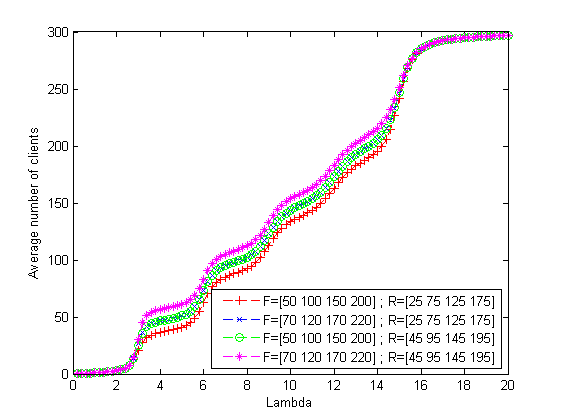
\includegraphics[width=0.45\textwidth, height=0.29\textwidth]{images/test1_fig2}
%\caption{Average number of clients in the system versus arrival rate ($\lambda$): $\mu=1$, $K=5$ and $B=300$}
%\label{fig:image-chap4-1_par_1-test1_fig2}
%\end{figure}

\begin{figure}[!ht]
\centering
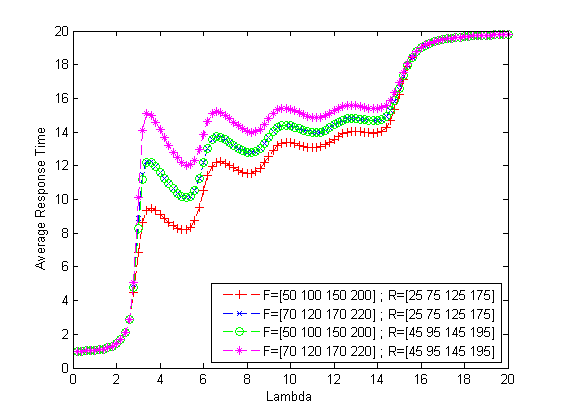
\includegraphics[width=0.45\textwidth, height=0.29\textwidth]{images/test1_fig1}
\caption{Average response time in the system versus arrival rate ($\lambda$): $\mu=1$, $K=5$ and $B=300$}
\label{fig:image-chap4-1_par_1-test1_fig1}
\end{figure}

\textbf{Experiment 2:} 
we analyse the behavior of the average number of servers (VMs) activations per time unit according to arrival rate 
(figures~\ref{fig:image-chap4-1_par_1_test2_fig1} and ~\ref{fig:image-chap4-1_par_1_test2_fig2}). We assume that the number of levels ($K$) $=$ 7, the system capacity ($B$) $=$ 250, $S_{1}=3$ 
and $S_{k+1}=S_{k}+3$ $\forall k$ (i.e. we activate three VMs when we switch from level $k$ to $k+1$). We let vary  the arrival rate $\lambda$ in X-axis. 
We performed tests for different values for thresholds $F$ and $R$. 
We assume in figure~\ref{fig:image-chap4-1_par_1_test2_fig1} a total overlap between the thresholds of activation $F$ and deactivation $R$, 
i.e. $R_1 < F_1 < R_2 < F_2 < R_3 < F_3 < R_4 < F_4 < R_5 < F_5 < R_6 < F_6$ and in figure~\ref{fig:image-chap4-1_par_1_test2_fig2} no overlap between the thresholds of activation $F$ and deactivation $R$, 
i.e. $R_1 < R_2 < R_3 < R_4 < R_5 < R_6 < F_1 < F_2 < R_3 < F_4 < R_5 < F_6$. 
Results (figure~\ref{fig:image-chap4-1_par_1_test2_fig1} and ~\ref{fig:image-chap4-1_par_1_test2_fig2}) show that thresholds values and the difference between activation and deactivation 
thresholds influence the shape of the curve of activation rate. We notice that more activation thresholds ($F$) are far from deactivation thresholds 
($R$) then less there are activations. Indeed, when thresholds are far from each other, 
we minimize oscillations between levels, which shows that it is interesting to use a hysteresis models for Cloud resources scaling.

\begin{figure}[!ht]
\centering
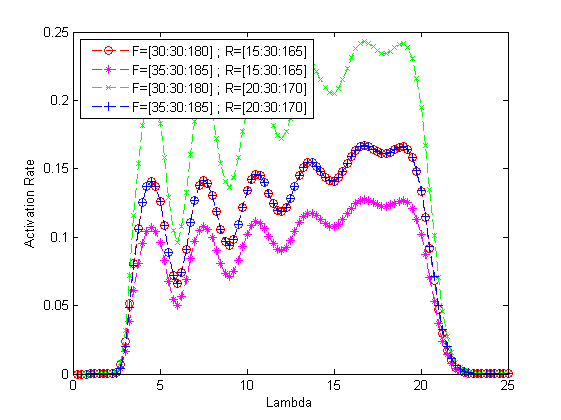
\includegraphics[width=0.45\textwidth, height=0.29\textwidth]{images/test2_fig1}
\caption{Activation rate versus arrival rate ($\lambda$): $\mu=1$, $K=7$ and $B=250$ (total overlap between activation and deactivation the thresholds)}
\label{fig:image-chap4-1_par_1_test2_fig1}
\end{figure}

\begin{figure}[!ht]
\centering
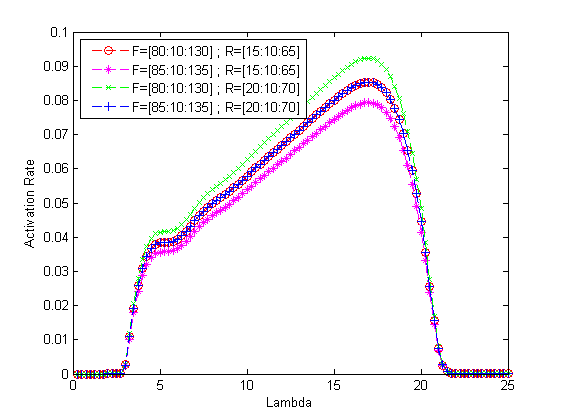
\includegraphics[width=0.45\textwidth, height=0.29\textwidth]{images/test2_fig2}
\caption{Activation rate versus arrival rate ($\lambda$) : $\mu=1$, $K=7$ and $B=250$ (no overlap between activation and deactivation thresholds)}
\label{fig:image-chap4-1_par_1_test2_fig2}
\end{figure}

\textbf{Experiment 3:} we analyse the overall cost (Figure~\ref{fig:image-chap4-1_par_1_test3_fig3}). we assume that the arrival rate ($\lambda$) $=$ 4, the number of levels ($K$) $=$ 7 and system capacity ($B$) $=$ 500, $S_{1}=3$ and 
$S_{k+1}=S_{k}+3$ $\forall k$ (i.e. we activate three VMs when we switch from level $k$ to $k+1$). We set $R=[45\mbox{ }95\mbox{ }145\mbox{ }195\mbox{ }245\mbox{ }295]$ and we vary in X-axis values of $F$. The initial value is $F_{init}=[50\mbox{ }100\mbox{ }150\mbox{ }200\mbox{ }250\mbox{ }300]$ (it corresponds to 0 in the x-axis) then we increase the values of $F$. For example, 10 in the X-axis corresponds to $F$ = $F_{init}+10=[50\mbox{ }100\mbox{ }150\mbox{ }200\mbox{ }250\mbox{ }300]+10$ $=$ [60 110 160 210 260 310]. We measure the overall cost for different values of $C_{A}$ (activationCost in Figure~\ref{fig:image-chap4-1_par_1_test3_fig3}). We notice that when $F$ increases the overall cost decreases in a first phase then increases after. The reason is that the formula of the overall cost includes both parameters that increases (for example: the average number of clients) and parameters that decreases (for example: the activation rate) according to $F$. The thresholds configuration that ensures the minimal cost depends on $C_{A}$ (activationCost).

\begin{figure}[!ht]
\centering
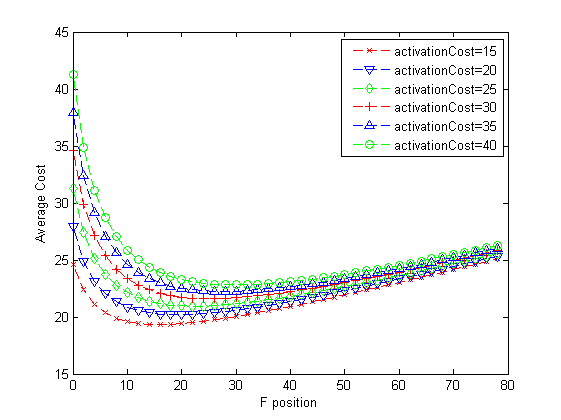
\includegraphics[width=3.1in]{images/test3_fig3}
\caption{Global cost versus $F$ values: $\lambda=4$,  $\mu=1$, $K=7$, $B=500$, $R=[45$ $95$ $145$ $195$ $245$ $295]$ and $F_{init}=[50\mbox{ }100\mbox{ }150\mbox{ }200\mbox{ }250\mbox{ }300]$}
\label{fig:image-chap4-1_par_1_test3_fig3}
\end{figure}

\textbf{Experiment 4:} we compare a model (\textbf{conf 1}) in which only one VM is activated/deactivated when we switch from one level to another  ($K=32$, $S_1=1$, $S_{k+1}=S_{k}+1$ $\forall k<K$, so $S_{K}=S_{32}=32$) and two models (\textbf{conf2}, \textbf{conf3}) in which many VMs are activated/deactivated when we switch from one level to another ($K=6$, $S_1=1$, $S_{k+1}=2*S_{k}$ $\forall k<K$, so $S_{K}=S_{6}=32$). The overall number of servers (VMs) for the three models is $C=32$ but we have less thresholds in \textbf{conf2} and \textbf{conf3}. In the experiment, we assume that the system capacity ($B$) $=$ 400 and we vary the arrivals rate ($\lambda$). Thresholds of \textbf{conf2} (respectively \textbf{conf3}) were chosen so that the associated model is an upper bound (respectively lower bound) for the performances of the model \textbf{conf1}. Values of F thresholds are illustrated in Figure~\ref{fig:fconfig} and we have $R_{k}=F_{k}-5$ $\forall k$ in all models. Figure~\ref{fig:image-chap4-comp_test1_fig1} illustrates the experiment results (the average number of clients of each model for different arrival rates ($\lambda$)). The result of \textbf{conf2}  (resp. \textbf{conf3}) is always greater (resp. smaller) to the one-by-one model (\textbf{conf1}). \textbf{conf2} and \textbf{conf3} have less thresholds than \textbf{conf1}, so faster to analyse. This idea is useful to analyse large one-by-one models in which we can analyse bounding and smaller models to find a lower and upper bounds for performance rather than analysing the large (so complex) original model.

\begin{figure}[!ht]
\centering
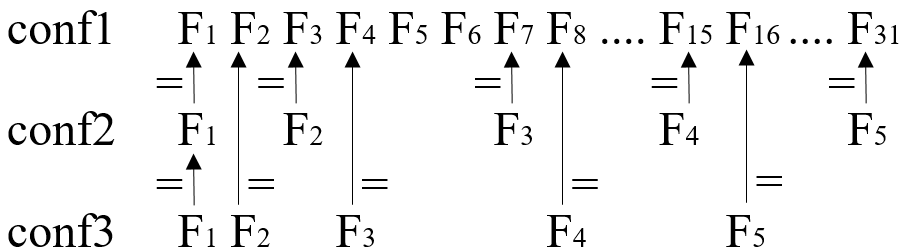
\includegraphics[width=0.45\textwidth, height=0.11\textwidth]{images/F_config}
\caption{The values of F for conf1, conf2 (upper bound) and conf3 (lower bound)}
\label{fig:fconfig}
\end{figure}

\begin{figure}[!ht]
  \centering
  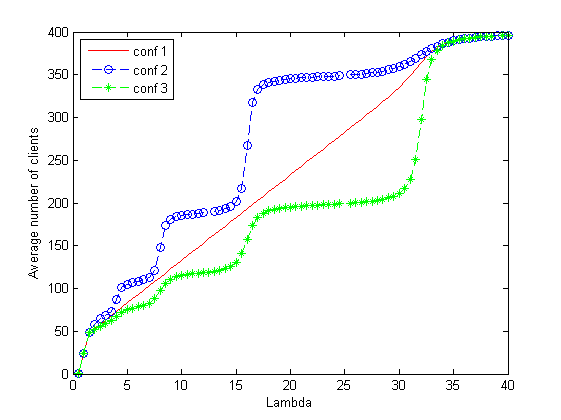
\includegraphics[width=0.45\textwidth, height=0.29\textwidth]{images/comp_test1_fig1}
  \caption{Average response time in the system versus arrival rate ($\lambda$): $\mu=1$, $B=400$, $32$ servers - Comparison of the three models -}
  \label{fig:image-chap4-comp_test1_fig1}
\end{figure}
%
% \section{Numerical results}
% We implemented the mathematical methods : (1) aggregation, (2) LDQBD, (3) balance equations, and we performed a set of experiments. In this section, we first present a comparison between the three methods in terms of resolution time. Then we give some numerical examples that aim to show the evolution of performance measures and cost according to arrival rate and thresholds values. All tests were implemented and performed on a machine with "Intel i7" CPU and 8GB of RAM.
%
% \subsection{Comparison between mathematical methods}
% Table~\ref{tab:Tableau-comparatif-methodes-res} shows the execution time of each mathematical method for different values of : K (the number of levels) and B (the capacity of the system). In the first line we have the smallest instance (K=5, B=300, markov chain with 521 stats), and in the last line we have the largest one (K=1000, B=75000, markov chain with 134921 stats). We observe that the method using the balance equations is the fastest among the three for all instances. Indeed, the calculation is made using formulas that contain basic operations. The aggregation method takes a lot of time for large chains. The reason is the complexity of the GTH approach that we use to resolve the generated sub chains. The method based on the LDQBD structure uses matrix inversion. For $K = 1000$ and $B = 75000$, the program returned an error "out of memory" because of the huge size of the matrix.
%
% \begin{table}[H]
% %\renewcommand{\arraystretch}{1.3}
% \caption{Comparison between mathematical methods in terms of execution time}
% \label{tab:Tableau-comparatif-methodes-res}
% \centering
% \begin{tabular}{ c | c c c}
%   - & \begin{tabular}{@{}c@{}} Agregation + GTH\end{tabular} & LDQBD & \begin{tabular}{@{}c@{}}Balance equations \end{tabular} \\
%   \hline
%   \begin{tabular}{@{}c@{}}K = 5 \\ B = 300 \\ (521 stats)\end{tabular} & 0.246 sec & 0.017 sec & 0.006 sec \\
%   \hline
%   \begin{tabular}{@{}c@{}}K = 10 \\ B = 750 \\ (1271 stats)\end{tabular} & 1.678 sec & 0.041 sec & 0.011 sec \\
%   \hline
%   \begin{tabular}{@{}c@{}}K = 50 \\ B = 3750 \\ (6671 stats)\end{tabular} & 89.010 sec & 0.496 sec & 0.095 sec \\
%   \hline
%   \begin{tabular}{@{}c@{}}K = 100 \\ B = 7500 \\ (13421 stats)\end{tabular} & 679.342 sec & 2.775 sec & 0.282 sec \\
%   \hline
%   \begin{tabular}{@{}c@{}}K = 500 \\ B = 37500 \\ (67421 stats)\end{tabular} & +30 min & 304.437 sec & 7.408 sec \\
%   \hline
%   \begin{tabular}{@{}c@{}}K = 1000 \\ B = 75000 \\ (134921 stats)\end{tabular} & +30 min & \begin{tabular}{@{}c@{}}"Out of memory"\\ (inversion of \\a very large matrix)\end{tabular} & 34.401 sec \\
% \end{tabular}
% \end{table}
%
% \subsection{Numerical Examples : Evaluation of performance and cost}
% In this section we consider a threshold-based queuing system with hysteresis and we present some numerical examples that aim observe the evolution of performance measures and cost.
%
% We first analyze the behavior of the average number of clients in the system (figure~\ref{fig:image-chap4-1_par_1-test1_fig2}) and the average response time (figure~\ref{fig:image-chap4-1_par_1-test1_fig1}). In these figures : the service rate ($\mu$) $=$ 1, the number of servers ($K$) $=$ 5, and system capacity ($B$) $=$ 400. In X-axis, we vary the arrival rate ($\lambda$). Y-axis in figure~\ref{fig:image-chap4-1_par_1-test1_fig2} (resp. figure~\ref{fig:image-chap4-1_par_1-test1_fig1}) represents the average number of clients in the system (resp. the average response time). We performed tests for different values for thresholds $F$ and $R$ (which is represented by the four curves). In figure~\ref{fig:image-chap4-1_par_1-test1_fig2}, the average number of clients increases when the arrival rate ($\lambda$) is bigger. The system is saturated when $\lambda$ reaches $5$. The reason is that above $\lambda=5$, we have $\frac{\lambda}  {K*\mu} >= 1$. If we compare the curves of figure~\ref{fig:image-chap4-1_par_1-test1_fig2} (resp. ~\ref{fig:image-chap4-1_par_1-test1_fig1}), we notice that more the threshold values are significant then more the average number of clients (resp. average response time) is considerable. i.e. when we choose larger thresholds, the servers are activated following a larger number of customers in the system, which results in less performance.
%
% \begin{figure}[ht]
% \centering
% 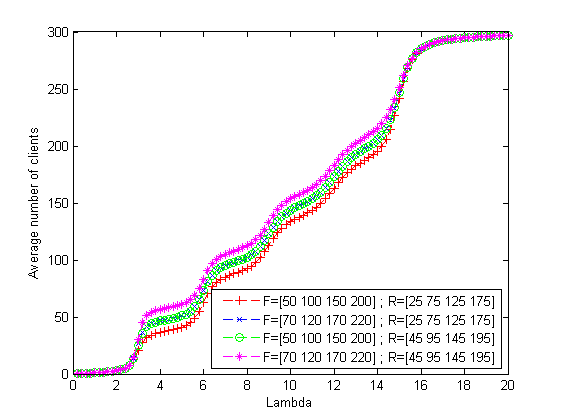
\includegraphics[width=3.5in]{images/test1_fig2}
% \caption{Average number of clients in the system versus arrival rate ($\lambda$) : $\mu=1$, $K=5$ and $B=400$}
% \label{fig:image-chap4-1_par_1-test1_fig2}
% \end{figure}
%
% \begin{figure}[ht]
% \centering
% 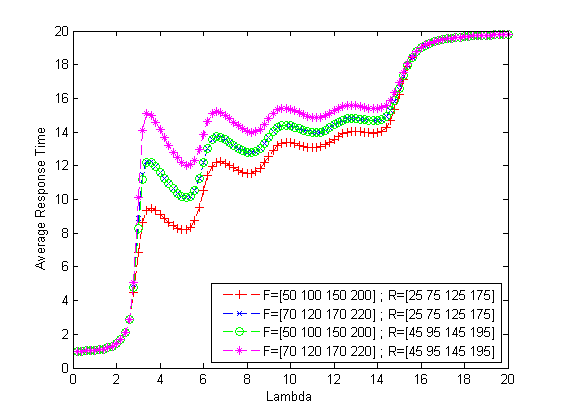
\includegraphics[width=3.5in]{images/test1_fig1}
% \caption{Average response time in the system versus arrival rate ($\lambda$) : $\mu=1$, $K=5$ and $B=400$}
% \label{fig:image-chap4-1_par_1-test1_fig1}
% \end{figure}
%
% We next analyze the behavior the average number of servers activations per time unit (figures~\ref{fig:image-chap4-1_par_1_test2_fig1}, ~\ref{fig:image-chap4-1_par_1_test2_fig2} and ~\ref{fig:image-chap4-1_par_1_test2_fig3}). In these figures : service rate ($\mu$) $=$ 1, the number of servers ($K$) $=$ 7, and system capacity ($B$) $=$ 250. In X-axis, we vary the arrival rate ($\lambda$).Y-axis represents activation rate (i.e. the average number of servers activations per time unit). We performed tests for different values for thresholds $F$ and $R$. The notation used to write thresholds in the figure is $F=[a:b:c]$ (with $a=F_1$, $c=F_{K-1}$ and $\forall i$ $b=F_{i+1}-F_{i}$). In figure~\ref{fig:image-chap4-1_par_1_test2_fig1}, we have a total overlap between the thresholds of activation $F$ and deactivation $R$ (i.e. $R_1 < F_1 < R_2 < F_2 < R_3 < F_3 < R_4 < F_4 < R_5 < F_5 < R_6 < F_6$). In figure~\ref{fig:image-chap4-1_par_1_test2_fig2} we have no overlap between activation and deactivation thresholds (i.e. $R_1 < R_2 < R_3 < R_4 < R_5 < R_6 < F_1 < F_2 < F_3 < F_4 < F_5 < F_6$ ). And finally for Figure~\ref{fig:image-chap4-1_par_1_test2_fig3}, we have a partial overlap between the activation and deactivation thresholds (i.e. $R_1 < R_2 < R_3 < F_1 < F_2 < F_3 < R_4 < R_5 < R_6 < F_4 < F_5 < F_6$). Results show that thresholds values and the difference between activation thresholds and deactivation thresholds influence the shape of the curve of activation rate. We notice that more activation thresholds ($F$) are far from deactivation thresholds ($R$) then less there are activations. Indeed, when thresholds are far from each other, we minimize oscillations between levels, which shows that it is interesting to use a hysteresis models for Cloud resources scaling.
%
% \begin{figure}[ht]
% \centering
% 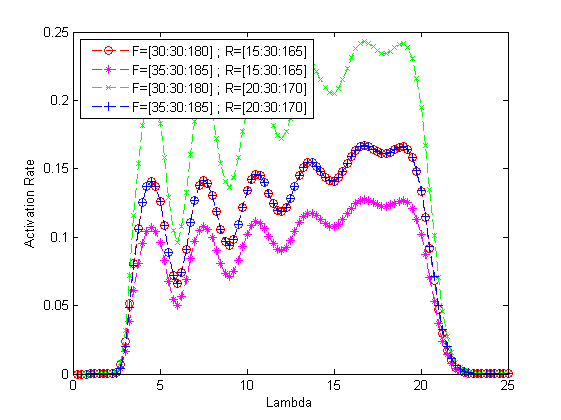
\includegraphics[width=3.5in]{images/test2_fig1}
% \caption{Activation rate versus arrival rate ($\lambda$) : $\mu=1$, $K=7$ and $B=250$ (total overlap between activation and deactivation the thresholds)}
% \label{fig:image-chap4-1_par_1_test2_fig1}
% \end{figure}
%
% \begin{figure}[ht]
% \centering
% 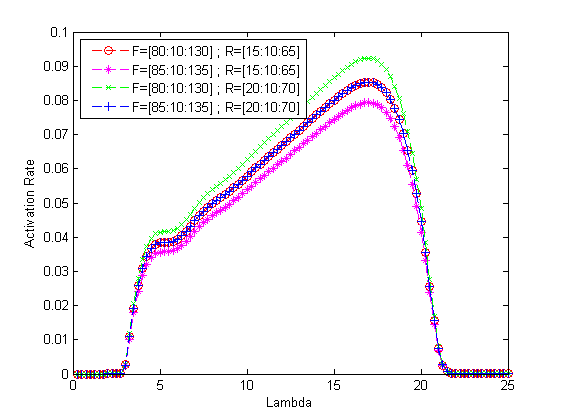
\includegraphics[width=3.5in]{images/test2_fig2}
% \caption{Activation rate versus arrival rate ($\lambda$) : $\mu=1$, $K=7$ and $B=250$ (no overlap between activation and deactivation thresholds)}
% \label{fig:image-chap4-1_par_1_test2_fig2}
% \end{figure}
%
% \begin{figure}[ht]
% \centering
% 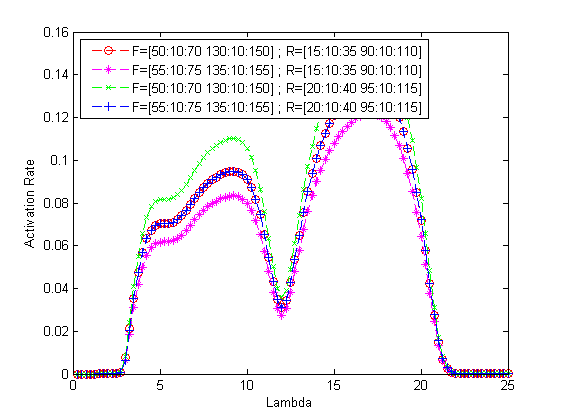
\includegraphics[width=3.5in]{images/test2_fig3}
% \caption{Activation rate versus arrival rate ($\lambda$) : $\mu=1$, $K=7$ and $B=250$ (partial overlap between the activation and deactivation thresholds)}
% \label{fig:image-chap4-1_par_1_test2_fig3}
% \end{figure}
%
% Finally we analyze the global cost (figure~\ref{fig:image-chap4-1_par_1_test3_fig3}). In this figure : service rate ($\mu$) $=$ 1, arrival rate ($\lambda$) $=$ 4, number of servers ($K$) $=$ 7 and system capacity ($B$) $=$ 500. We set $R=[45\mbox{ }95\mbox{ }145\mbox{ }195\mbox{ }245\mbox{ }295]$ and we vary in X-axis values of $F$. The initial value is $F_{init}=[50\mbox{ }100\mbox{ }150\mbox{ }200\mbox{ }250\mbox{ }300]$ (it corresponds to 0 in the x-axis) then we increase the values of $F$. For example, 10 in the X-axis corresponds to $F$ = $F_{init}+10=[50\mbox{ }100\mbox{ }150\mbox{ }200\mbox{ }250\mbox{ }300]+10$ $=$ [60 110 160 210 260 310]. We measure the global cost for different values of $C_{A}$ (activationCost in the figure). We notice that when $F$ increases the global cost decreases in a first phase then increases after. The reason is that the formula of the global cost includes both the average number of clients that increases and the activation rate that decreases. The thresholds configuration that ensures the minimal cost depends on $C_{A}$ (activationCost).
%
% \begin{figure}[ht]
% \centering
% 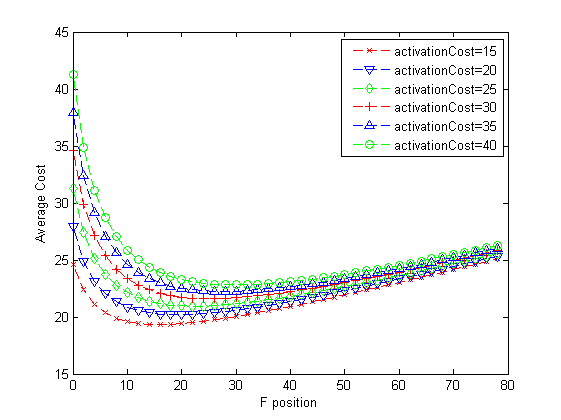
\includegraphics[width=3.5in]{images/test3_fig3}
% \caption{Global cost versus $F$ values : $\lambda=4$,  $\mu=1$, $K=7$, $B=500$, $R=[45$ $95$ $145$ $195$ $245$ $295]$ and $F_{init}=[50\mbox{ }100\mbox{ }150\mbox{ }200\mbox{ }250\mbox{ }300]$}
% \label{fig:image-chap4-1_par_1_test3_fig3}
% \end{figure}

\section{Conclusion}

We develop numerical and analytical methods for the analysis of a hysteresis queueing system modelling a cloud system with activation/deactivation of block of VMs. 
We give numerical values even in the case of large Markov chains, for both performance and energy consumption measures, and we analyze the impact of the thresholds.  One another important contribution of this paper  is to suppose fewer constraints on the thresholds in order to analyze the impact on  mean number of activations/deactivations.
We define a
global cost for performance and energy consumption in order to propose  a trade off between performance and energy consumption.
As a future,  we propose to develop optimization algorithms in order to obtain the thresholds with minimize
the overall cost.


%Moreover, the bounding models presented in the paper are also interesting and allow to reduce the complexity of the threshold-based queue with hysteresis.





%we observe clearly that when we apply stochastic bounds for batch-arrival distribution, we
%derive also bounds on performance measures and those in relatively less time. And even if a reduction applied on the batch-arrival distribution may seem important (from $500$ states to only $10$ states or $50$ states) the results on performance metrics are, however, very close to the exact results and very accurate. Regarding the computation times, we can remark that for $\rho\simeq 0.2$  we have tended to divide by $9$ the execution time when we reduce the size of the batch-arrival distribution to $bins=50$ and by a little more than $6$ when $\rho\simeq 0.96$, which is quite important given the interesting results obtained.

%We also note that the use of bounding models (Upper bound model and Lower bound model) can also be another way of defining stochastic bounds on performance measurements of the hysteresis model with reduced complexity.



%
%To conclude, through these examples, we show that the results provided after using the stochastic bounds on the batch-arrival distribution, are very accurate and gives a good coverage of the results of the threshold-based queue with hysteresis, and those with considerably reduced computation times.
%Moreover, the bounding models presented in the paper are also interesting and allow to reduce the complexity of the threshold-based queue with hysteresis.
%
%
%



% use section* for acknowledgment
%\section*{Acknowledgment}
%
%
%The authors would like to thank...





% trigger a \newpage just before the given reference
% number - used to balance the columns on the last page
% adjust value as needed - may need to be readjusted if
% the document is modified later
%\IEEEtriggeratref{8}
% The "triggered" command can be changed if desired:
%\IEEEtriggercmd{\enlargethispage{-5in}}

% references section

% can use a bibliography generated by BibTeX as a .bbl file
% BibTeX documentation can be easily obtained at:
% http://mirror.ctan.org/biblio/bibtex/contrib/doc/
% The IEEEtran BibTeX style support page is at:
% http://www.michaelshell.org/tex/ieeetran/bibtex/
\bibliographystyle{IEEEtran}
% argument is your BibTeX string definitions and bibliography database(s)
\bibliography{references}
%
\end{document} 